% Объединение возможностеи
\label{collective_global}

Если оценку параметров объектов $x_{ij}$ для задачи выбора объектов (см. раздел~\ref{selection_task}) совершают несколько экспертов, исходным материалом для программного комплекса служат оценки 
\begin{equation}
\label{Psetlargedef}
	\Pi_{ij} = \{\p^{(r)}\}_{ij}, i = \dotN, j = \dotM, r = \dotR, 
\end{equation}
где $r$ --- номер эксперта, $i$ --- номер объекта, $j$ --- номер параметра объекта. На вход алгоритма выбора объектов подаются только экспертное  мнение одного эксперта (см. рис.~\ref{ris:program_global}) $\p_{ij},  i = \dotN, j = \dotM$,  поэтому в настоящем разделе ставятся задачи сведения набора $\Pi_{ij}$ к $\p_{ij}$ для всех $i = \dotN, j= \dotM$ --- задачи нахождения  оценок, выражающих коллективное мнение экспертов, или, короче говоря, задачи <<коллективной экспертизы>>. 

\begin{figure}[h]
\center{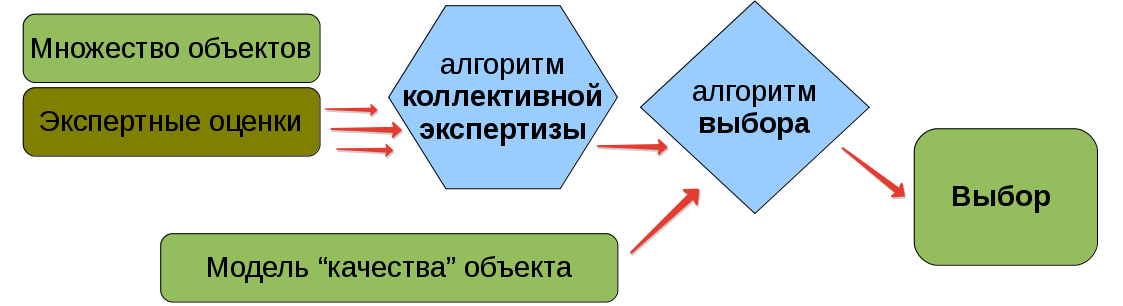
\includegraphics[width=0.85\linewidth]{./pic/globalscheme}}  
\caption{\small Схема, иллюстрирующая работу программного комплекса в режиме нахождения наиболее <<качественных>> объектов на выходе по мнениям нескольких экспертов и модели <<качества>> объектов (функции $f: x = f(x_1, x_2, ...)$) на входе. }
\label{ris:program_global}
\end{figure}

Задача коллективной экспертизы в рамках использования модели нечётких оценок в теории возможностей Пытьева может быть поставлена и решена различными методами:
	\begin{enumerate}
		\item Методы <<евклидовой близости к среднему>>~\cite{pytyev_experts}: метод матриц попарных сравнений, векторов перестановок, векторов предпочтений и др.;
		\item Новый метод -- введение отношения квазипорядка~\ref{preorder_pyt}  на множестве возможностных распределений нечётких  элементов $\tilde x_{ij}$ (см. раздел~\ref{selection_task}) и вычисление верхней (нижней) грани или точной верхней (нижней) грани каждого из множеств~\ref{Psetlargedef} экспертных оценок от разных экспертов, отдельно для каждого $i = \dotN, j= \dotM$.
	\end{enumerate} 
	
\subsection{Методы <<евклидовой близости к среднему>>}


	
\subsubsection{Метод матриц попарных сравнений}


\subsubsection{Метод векторов предпочтений}


\subsection{Метод вычисления верхних граней множеств экспертных оценок}

\subsubsection{Квазипорядок на множестве возможностных распределений}
\label{preorder_pyt}

Определение квазипорядка аналогично определению порядка \eqref{interv_order}, за исключением отсутствия требования равенства в качестве эквивалентности~\cite{Mirkin}: 
 \begin{equation}
\label{preoder_def}
\begin{split}
\forall A: & A \prec A; \\
\forall A, B, C: & A \prec B \text{ и } B \prec C \Rightarrow A \prec C.
\end{split}
\end{equation}

На множестве возможностных распределений, определённых на (одном и том же, фиксированном) множестве $X$, то есть на множестве функций $\p(\cdot):\ X\to[0,1]$, таких что $\sup_{x\in X} \p(x) = 1$, введём отношение~<<$\prec$>>: $\p_1\prec\p_2$, если:
\begin{enumerate}
    \item\label{order-D1}
        носитель $\p_1(\cdot)$ меньше (по включению), чем носитель $\p_2(\cdot)$: $\supp\p_1\subset\supp\p_2$;
    \item\label{order-D2}
        найдётся непрерывная строго монотонная функция ${\gamma(\cdot):\ [0,1]\to[0,1]}$, $\gamma(0) = 0$, $\gamma(1) = 1$, такая что $\p_2(x) = \gamma(\p_1(x))$ при $x\in\supp\p_1$;
    \item\label{order-D3}
        значения распределения $\p_2(\cdot)$ на носителе распределения $\p_1(\cdot)$ не меньше, чем значения $\p_2(\cdot)$ вне носителя $\p_1(\cdot)$:
        $$\inf\{\p_2(x) \mid x\in\supp\p_1\} \geqs \sup\{\p_2(x) \mid x\in X\setminus\supp\p_1\};$$
\end{enumerate}
где $\supp \p_i = \{x\in X:\ \p_i(x) > 0\}$~--- носитель распределения $\p_i(\cdot),\ i=1,\, 2$.

В ходе выполнения работы показано, что отношение <<$\prec$>> является отношением квазипорядка, то есть рефлексивно и транзитивно. При этом из $\p_1\prec\p_2$ и $\p_2\prec\p_1$ не следует тождественное равенство $\p_1(\cdot)$ и $\p_2(\cdot)$, однако из этого следует эквивалентность возможностных распределений $\p_1(\cdot)$ и $\p_2(\cdot)$, то есть существование непрерывной строго монотонной функции $\gamma(\cdot):\ [0,1]\to[0,1]$, $\gamma(0) = 0$, $\gamma(1) = 1$, такой что $\p_2(x) = \gamma(\p_1(x))$ при $x\in X$.

В случае, если распределения $\p_1(\cdot)$ и $\p_2(\cdot)$ сравнимы, то есть $\p_1\prec\p_2$ или $\p_2\prec\p_1$, будем говорить, что эти распределения не противоречат друг другу,
а запись $\p_1\prec\p_2$ будем читать как <<$\p_1$ уточняет $\p_2$>>.
Это связано с интерпретацией квазипорядка <<$\prec$>> как отношения, упорядочивающего возможностные распределения по степени их информативности. Такая интерпретация может быть проиллюстрирована тем, что всякое распределение, достигающее значения 1 в точке $x_0$, уточняет тривиальное распределение, тождественно равное единице, и одновременно с этим уточняется <<дельтобразным>> распределением, принимающим значение 1 в точке $x_0$ и значение 0 во всех остальных точках области определения.

\section{Содержательная интерпретация квазипорядка на множестве возможностных распределений}

Строгое обоснование содержательной интерпретации отношения <<$\prec$>> основано на его роли в следующей задаче принятия решений.

Пусть $\eta$ и $\zeta$~--- нечёткие элементы со значениями в $Y$ и $Z$ соответственно, совместное распределение возможностей которых есть $\p(\cdot):\ Y\times Z\to[0,1]$, и по реализации $y\in Y$ элемента $\eta$ требуется принять решение о реализации $z\in Z$ элемента $\zeta$. Множество чётких стратегий, минимизирующих возможность ошибки при $\p(\cdot) = \p_1(\cdot)$, обозначим $D_1$, при $\p(\cdot) = \p_2(\cdot)$~--- $D_2$.
В ходе выполнения работы доказана следующая теорема.

\begin{theorem}
\label{theorem_zubyuk}
    Пусть $\p_1\prec\p_2$, и множества $D_1$ и $D_2$ не пусты. Тогда при $\p(\cdot) = \p_1(\cdot)$ всем стратегиям из $D_1$ соответствует либо ненулевая возможность ошибки, при этом $D_1\subset D_2$, либо нулевая возможность ошибки, при этом для всякой $d_1\in D_1\setminus D_2$ найдётся такая стратегия $d_1'\in  D_1\cap D_2$, что возможность несовпадения решений, принятых с использованием $d_1$ и $d_1'$, равна нулю.
\end{theorem}

Рассмотрим подробно смысл данной теоремы. Итак, если всякой стратегии из множества $D_1$ соответствует ненулевая возможность ошибки, то $D_1\subset D_2$, то есть использование распределения $\p_1(\cdot)$ вместо $\p_2(\cdot)$ позволяет сузить множество оптимальных стратегий. Это в полной мере согласуется с трактовкой отношения $\p_1\prec\p_2$ как выражения того, что распределение $\p_1(\cdot)$ не менее информативно, чем $\p_2(\cdot)$: чем более информативно распределение, тем более конкретный ответ (более узкое множество оптимальных стратегий) оно позволяет получить в задаче принятия решений.

В случае, если всем стратегиям из множества $D_1$ соответствует нулевая возможность ошибки,
множество $D_1$, вообще говоря, не уже, чем множество $D_2$.
Однако для всякой стратегии $d_1\in D_1\setminus D_2$ в этом случае найдётся эквивалентная ей стратегия $d_1'\in D_1\cap D_2$; эквивалентность здесь понимается как равенство нулю возможности несовпадения принятых с использованием $d_1$ и $d_1'$ решений при $\p(\cdot) = \p_1(\cdot)$.
Таким образом, пополнение множества оптимальных стратегий при использовании распределения $\p_1(\cdot)$ вместо $\p_2(\cdot)$ может быть связано исключительно с тем, что некоторые элементарные исходы, имеющие ненулевую возможность при $\p(\cdot) = \p_2(\cdot)$, имеют нулевую возможность при $\p(\cdot) = \p_1(\cdot)$. Только при реализации таких исходов эквивалентные стратегии из множеств $D_1\setminus D_2$ и $D_1\cap D_2$ приводят к принятию разных решений.
Однако тот факт, что некоторые элементарные исходы, имеющие ненулевую возможность при $\p(\cdot) = \p_2(\cdot)$, имеют нулевую возможность при $\p(\cdot) = \p_1(\cdot)$ как раз и означает, что распределение $\p_1(\cdot)$ более информативно, чем $\p_2(\cdot)$: распределение $\p_1(\cdot)$ более конкретно, более чётко определяет исход эксперимента, так как множество возможных исходов при $\p(\cdot) = \p_1(\cdot)$ уже, чем при $\p(\cdot) = \p_2(\cdot)$.	
	
\subsubsection{Супремум и инфинум возможностных распределений. Алгоритм вычисления супремума}
\label{algo_sup_poss}

Для любой пары распределений $\p_1(\cdot)$ и $\p_2(\cdot)$ распределение $\p_1\vee\p_2(\cdot)$ определим как их супремум (если он существует), то есть как наиболее информативное среди всех распределений, уточняемых обоими распределениями $\p_1(\cdot)$ и $\p_2(\cdot)$. Распределение $\p_1\wedge\p_2(\cdot)$ определим как инфимум $\p_1(\cdot)$ и $\p_2(\cdot)$ (если он существует), то есть как наименее информативное среди всех распределений, уточняющих $\p_1(\cdot)$ и $\p_2(\cdot)$.

В ходе выполнения работы показано, что в случае, если область определения возможностных распределений конечна, супремум существует для любой пары распределений.  Тогда множество всех распределений образует полурешётку с идемпотентной, коммутативной, ассоциативной и дистрибутивной алгебраической операцией <<$\vee$>>, см. рис.~dummy. 
\begin{notive}
В случае, если область определения возможностных распределений конечна, инфимум тоже существует для любой пары распределений, если множество всех распределений пополнено функцией $0(\cdot)$, тождественно равной нулю на всей области определения (заметим, что с формальной точки зрения такая функция не является возможностным распределением, так как не найдётся точки, возможность которой равна 1). Более того, в ходе выполнения работы показано, что какой бы ни была область определения возможностных распределений, пополнение множества распределений функцией $0(\cdot)$ является необходимым условиям существования инфимума для любой пары распределений. Если для любой пары возможностных распределений существуют и супремум и инфимум, , множество всех распределений, пополненное $0(\cdot)$, образует решётку с алгебраическими операциями <<$\vee$>> и <<$\wedge$>>, являющимися идемпотентными, коммутативными, ассоциативными и дистрибутивными.
\end{notice}

Доказана система теорем, позволившая разработать численный метод построения супремума возможностных распределений и его компьютерную реализацию. А именно, алгоритм постоения супремума выглядит так.
dummy

\subsubsection{Супремум как коллективное мнение экспертов}

Теоретико-возможностная модель всех параметров всех объектов в задаче выбора определяется распределением $\p(\cdot):\ X\to[0,1]$ нечёткого вектора $\theta = \tetavector$, заданным формулой~\ref{p_theta_def}. Пусть из разных источников (от разных экспертов) получена информация, выраженная распределениями 
\begin{equation*}
	\p_r \big(\tvector\big) =  \inf_{i, j}\,\p^{(r)}_{ij}(x_{ij}), 
\end{equation*}
и на основе этой информации должно быть построено неизвестное распределение $\p$, являющееся по отношению к экспертным мнениям $\{\p_r\}$ коллективным мнением экспертов. 

Пусть множество всех распределений нечёткого элемента$\theta$, образует полурешётку с алгебраической операцией <<$\vee$>> (см. раздел~\ref{algo_sup_poss}). Поскольку операция <<$\vee$>> транзитивна и ассоциативна, можно, не ограничивая общности, положить $R = 2$, и тогда качестве коллективной экспертизы можно взять распределением $\p_1 \vee\p_2(\cdot)$, пользуясь алгоритмом из раздела~\ref{algo_sup_poss}. Рассмотрим содержательную сторону этого подхода.



Первый подход является математическим выражением принципа недоверия источникам информации. Он может быть применён в том случае, если хотя бы одно из распределений $\p_1(\cdot)$ и $\p_2(\cdot)$ уточняется распределением $\p(\cdot)$. То есть если информация, полученная из одного из источников, может противоречить истине, но при этом информация из другого источника истине не противоречит, но, вообще говоря, не полна. Покажем, что в этом случае означает использование распределения $\p_1\vee\p_2(\cdot)$ вместо $\p(\cdot)$ на примере задачи принятия решения о реализации $t$ нечёткого элемента $\theta$ по реализации $y$ нечёткого элемента $\eta$, рассмотренной выше. Обозначим $D$, $D_1$, $D_2$ и $D'$~--- множества стратегий, оптимальных в рамках моделей, определяемых распределениями $\p(\cdot)$, $\p_1(\cdot)$, $\p_2(\cdot)$ и $\p_1\vee\p_2(\cdot)$ соответственно. При выполнении указанных условий $\p\prec\p_1\vee\p_2$, $\p_1\prec\p_1\vee\p_2$ и $\p_2\prec\p_1\vee\p_2$. Пусть, для определённости, $D\subset D'$, $D_1\subset D'$ и $D_2\subset D'$, см. теорему~\ref{theorem_zubyuk}. Это означает, что множество $D'$ содержит все стратегии, оптимальные в рамках истинной модели. Однако кроме них она содержит также все стратегии, оптимальные в рамках моделей, соответствующих информации, полученной из обоих источников. То есть в множество $D'$ включаются все стратегии, оптимальные хотя бы для одного из $\p_i(\cdot),\ i=1,\, 2$, а те стратегии, которые нет оснований включить в множество $D'$ (с учётом информации, полученной из двух рассматриваемых источников), в него не включаются.

Второй подход является математическим выражением принципа доверия источникам информации. Он может быть применён в том случае, если оба распределения $\p_1(\cdot)$ и $\p_2(\cdot)$ уточняются распределением $\p(\cdot)$. То есть если информация из обоих источников не противоречит истине, но, вообще говоря, не полна. Как и выше, покажем, что в этом случае означает использование распределения $\p_1\wedge\p_2(\cdot)$ вместо $\p(\cdot)$ на примере задачи принятия решения о реализации $t$ нечёткого элемента $\theta$ по реализации $y$ нечёткого элемента $\eta$.
Обозначим $D$, $D_1$, $D_2$ и $D'$~--- множества стратегий, оптимальных в рамках моделей, определяемых распределениями $\p(\cdot)$, $\p_1(\cdot)$, $\p_2(\cdot)$ и $\p_1\wedge\p_2(\cdot)$ соответственно. При выполнении указанных условий $\p\prec\p_1\wedge\p_2$, $\p_1\wedge\p_2\prec\p_1$ и $\p_1\wedge\p_2\prec\p_2$. Пусть, для определённости, $D\subset D'$ и $D'\subset D_1\cap D_2$, см. теорему~\ref{theorem_zubyuk}.
Это означает, что множество $D'$ содержит все стратегии, оптимальные в рамках истинной модели. При этом в множество $D'$ включаются только те стратегии, которые оптимальны для обоих распределений $\p_1(\cdot)$ и $\p_2(\cdot)$, то есть все те стратегии, которые нет оснований не включить в $D'$ (с учётом информации, полученной из двух рассматриваемых источников).
